\documentclass[variant=courcework]{bsuir}

\faculty{компьютерного проектирования}
\departmentlong{инженерной психологии и эргономики}
\departmentshort{эргономики}
\manager{эргономики}
\worktitle{Создание сервиса поиска визуально схожих изображений в
неорганизованных коллекциях}
\workcode{БГУИР КР 1-58 01 01 002 ПЗ}
\titleright{Студент\\Руководитель}
\titleleft{Бородин А.Н.\\Кабариха В.А.}
\titlepageyear{2024}

\begin{document}

\maketitle

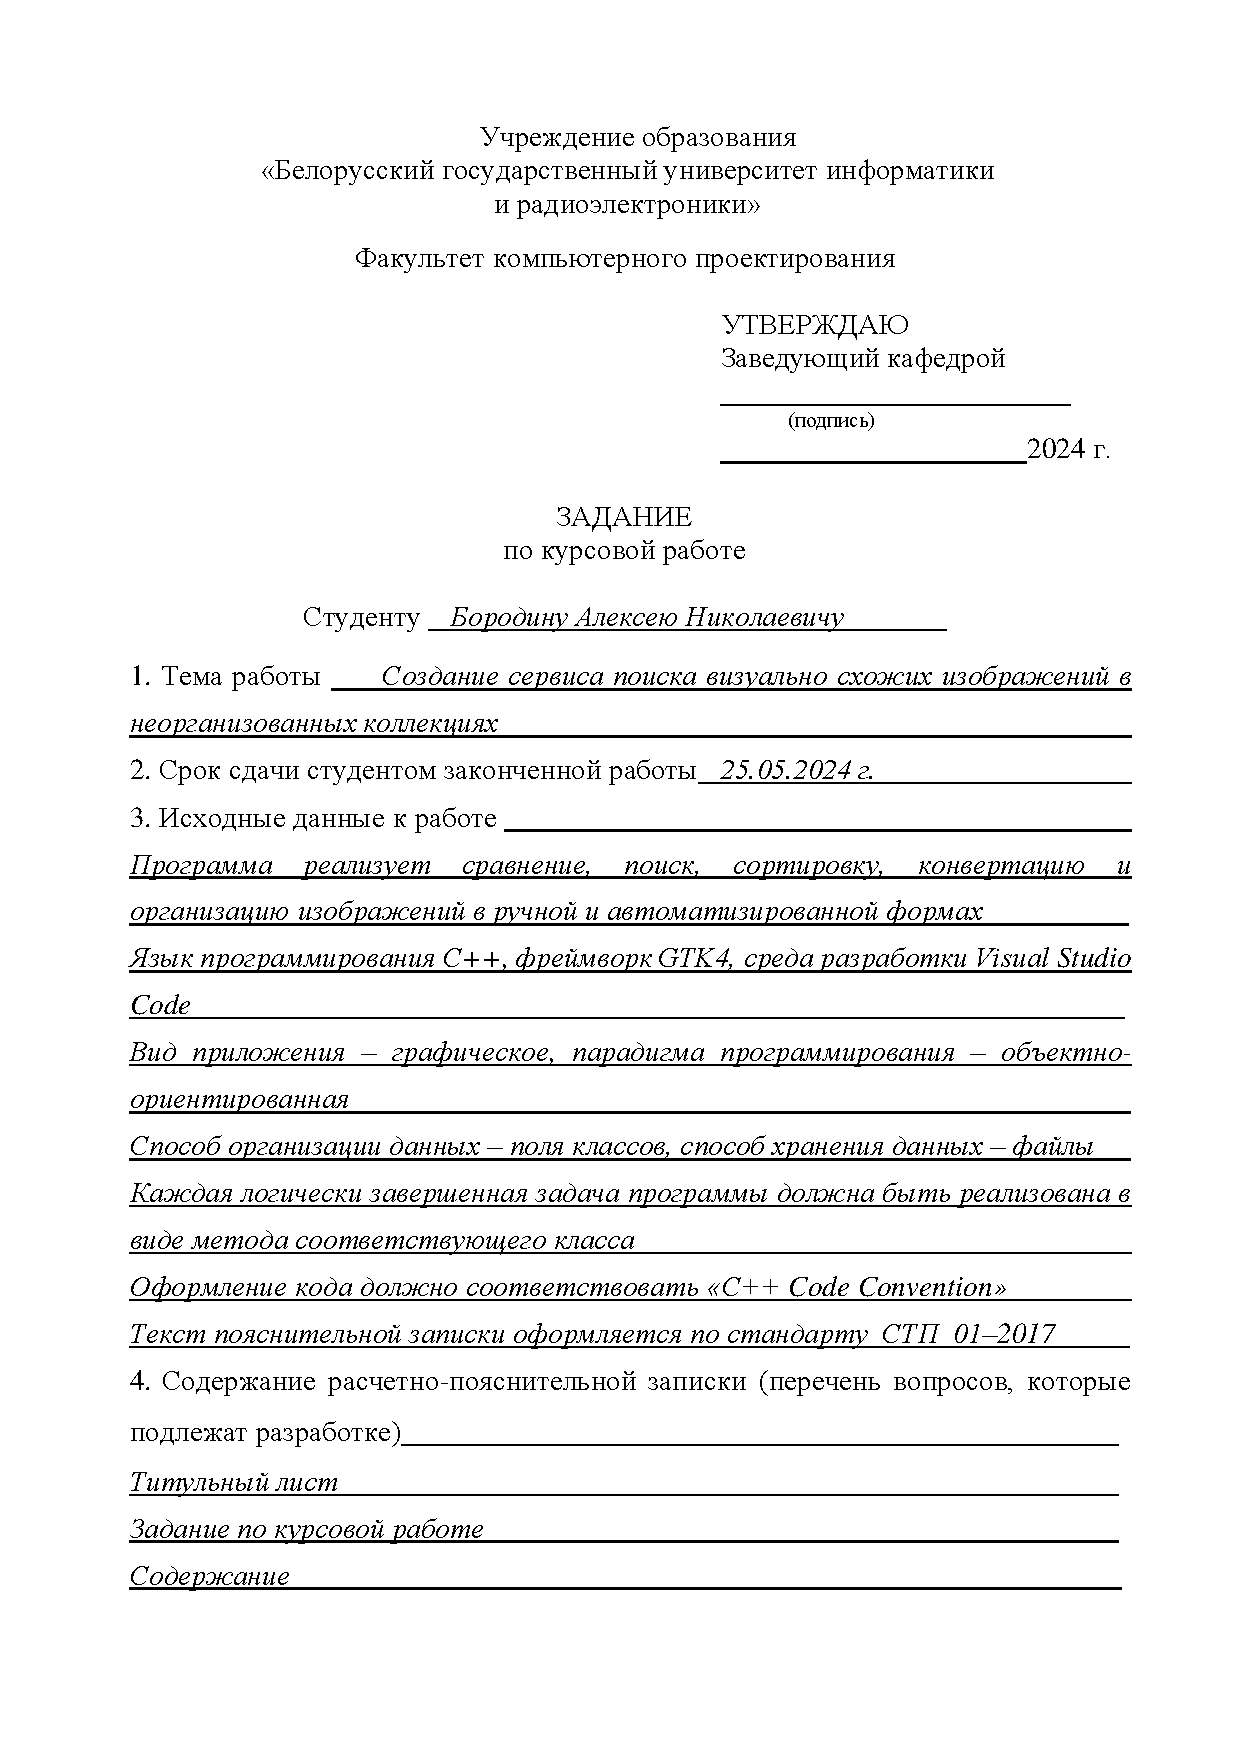
\includepdf[pages=-]{task.pdf}

\tableofcontents

\chapter*{Введение}

В современном мире объемы данных, включая изображения, растут с каждым днем.
Однако, с ростом количества данных возникает проблема поиска и классификации
информации. Визуальный поиск изображений становится особенно актуальным,
поскольку он позволяет пользователям находить изображения на основе их
визуальных характеристик, не зависимо от их текстового описания или тегов.

Сравнение изображений -- это процесс анализа двух или более изображений для
определения различий между ними. Это может включать в себя сопоставление
визуального содержания, такого как формы, цвета и текстуры, а также
использование алгоритмов для выявления изменений или аномалий. Сравнение
изображений широко используется в различных областях, включая цифровую
фотографию, медицинскую визуализацию, спутниковую разведку и системы
безопасности.

Целью данной курсовой работы является создание сервиса поиска визуально схожих
изображений в неорганизованных коллекциях на основе их визуальных характеристик,
таких как цвет, форма, текстура и других, даже если у них нет каких"=либо
метаданных, будь то теги или описание, который должен реализовать эффективную
систему индексации и хранения изображений, чтобы обеспечить быстрый доступ к ним
в коллекции и пользовательский интерфейс, который позволит пользователям
создавать выборки рассматриваемых файлов, следить за прогрессом сравнения и
просматривать результаты.

Данная работа будет включать в себя сравнительный анализ существующих решений,
оценочный выбор оптимальных инструментов для решения задачи, а также описание
разработанного сервиса. Будут представлены методы и алгоритмы, использованные
для сравнения изображений, описана система индексации и хранения данных, а также
представлен пользовательский интерфейс и результаты тестирования.

Ожидается, что результаты работы смогут применяться в реальных сценариях, где
требуется быстрый и точный поиск визуально схожих изображений в больших
коллекциях.

\chapter{Постановка задачи}

\section{Описание предметной области}

% Поиск и сравнение изображений
%     Методы поиска и идентификации похожих или дубликатных изображений в коллекции
%     Алгоритмы ранжирования и сортировки результатов поиска по степени визуального сходства
%     Способы визуализации и представления результатов сравнения изображений

% Управление коллекциями изображений
%     Методы организации и структурирования неорганизованных коллекций изображений
%     Подходы к классификации, группировке и кластеризации изображений на основе визуальных признаков
%     Механизмы для добавления, удаления и обновления изображений в коллекции

% Практические применения
%     Использование сервиса для поиска дубликатов и похожих изображений в личных или корпоративных коллекциях
%     Применение в задачах каталогизации, архивирования и управления медиаконтентом
%     Интеграция с другими системами, такими как системы управления контентом, электронные библиотеки и т.д.

\subsection{Область применения}
Визуальное сравнение изображений представляет собой двухэтапный процесс: сначала
проводится сравнение изображений, результатом которой являются некоторые
параметры, а затем, на их основе, дается оценка схожести. 

является важной технологией, находящей широкое
применение в различных сферах деятельности. Эта технология позволяет решать
широкий спектр практических задач, связанных с анализом, мониторингом и
интерпретацией визуальной информации.

\subsubsection{Безопасность}
Одной из ключевых областей применения визуального сравнения изображений является
обеспечение безопасности и проведение наблюдения. Данная технология используется
для обнаружения изменений на охраняемых объектах, идентификации людей и
транспортных средств, мониторинга критической инфраструктуры, а также для
анализа видеонаблюдения в реальном времени с целью выявления аномалий и
подозрительной активности.

\subsubsection{Медицина}
В медицинской сфере визуальное сравнение изображений играет важную роль в
отслеживании прогрессирования или регрессии заболеваний, выявлении ранних
признаков патологий, оценке эффективности лечения, а также в автоматизированном
скрининге и диагностике на основе сравнения с базами данных типичных патологий.

\subsubsection{Промышленность}
Промышленность и производство также широко используют технологию визуального
сравнения изображений для контроля качества продукции, мониторинга
производственных процессов, отслеживания износа и повреждений оборудования, а
также для контроля качества упаковки и маркировки.

\subsubsection{Применение в быту}
Сравнение изображений применяется и в быту. Пользователи ищут по изображениям
именования заинтересовавших их предметов и желаемых товаров, местоположения
локаций и имена людей, изображенных на фотографиях, названия фильмов, передач и
сериалов по кадрам из них.

\subsubsection{Авторское право}
Кроме того, визуальное сравнение изображений находит применение в сфере
интеллектуальной собственности и авторского права. Эта технология используется
для поиска дубликатов и похожих изображений в больших базах данных,
классификации и каталогизации коллекций изображений, отслеживания использования
защищенных изображений в Интернете и выявления случаев плагиата.

\subsubsection{Метрики}
Метрики же наоборот, высокоэкономичны, однако, уязвимы. К примеру, наиболее
популярная метрика, Индекс Структурного Сходства (SSIM), теряет смысл на
обрезанных и перевернутых изображениях. Для решения ее проблем было разработано
множество модификаций, но не одну нельзя назвать достаточно надежной: MS-SSIM,
3-SSIM, DSSIM, CW-SSIM, SSIMPLUS, cSSIM, SSIMULACRA, SSIMULACRA2, G-SSIM.
Однако, если точность не имеет особого значения, они очень полезны. Для
примитивных сравнений есть упрощенные оценки: пиковое отношение сигнала к шуму
(PSNR) и среднеквадратичная ошибка (MSE).

\subsection{Методики сравнения}
Можно выделить три основных подхода к сравнению изображений: метрики
структурного анализа, хеширование изображений и использование машинного
обучения.

\subsubsection{Машинное обучение}
Нейросетевые методы позволяют извлекать и сравнивать высокоуровневые визуальные
признаки, что дает значительные преимущества по сравнению с традиционными
методами. Они несравнимо больше аппаратных ресурсов чем метрики, однако
гарантируют большую точность и позволяют сравнивать смысловое содержание
изображений: одинаковый ли объект (тип объектов) на них изображен и на сколько
они похожи.

Сети для извлечения дескрипторов обучаются извлекать компактные числовые
дескрипторы, описывающие визуальные характеристики изображений. Примером таких
сетей служит \textit{ResNet}\cite{simonyan2015deep}.

Сиамские нейронные сети состоят из двух или более идентичных подсетей, которые
обрабатывают несколько изображений параллельно; их обучают определять, являются
ли два изображения похожими или нет, на основе сравнения их внутренних
представлений \cite{Koch2015SiameseNN}.

Сети с контрастивным обучением используют методы контрастивного обучения для
различения похожих и непохожих изображений путем сравнения их внутренних
признаков, подобные \textit{SimCLR}\cite{DBLP:journals/corr/abs-2002-05709}.

Сети для семантической сегментации, такие как
\textit{U-Net}\cite{10.1007/978-3-319-24574-4_28}, могут использоваться для
сравнения структуры и содержания изображений на основе сегментированных
областей.

Генеративные модели, например \textit{DCGAN}\cite{radford2015unsupervised},
могут применяться для сравнения изображений путем сравнения их внутренних
представлений.

\subsubsection{Хеширование}
Оптимальным в этой ситуации оказывается хеширование. Все алгоритмы хеширования
схожи: уменьшение размера, преобразование цветов, преобразования матрицы и
сравнение с другим хешем. В случае самого известного, перцептивного хеша:
уменьшение до 64 пикселей, обесцвечивание, замена каждого элемента на результат
его сравнения со средним значением по матрице и сравнение хешей через поиск
расстояния Хэмминга. Также популярны: по среднему значению блока, по цветовым
моментам, по преобразованию Радона, по среднему, по Марру-Гилдрету.

\section{Сравнительный анализ}

\subsection*{\textquote{rmlint}}

На рисунке \ref{img:rmlint.png} приводится пример вывода \textquote{rmlint},
консольной программы для поиска дубликатов общего предназначения. Для сравнения
файлов используется хеш-функция blake2b. Дополнительные варианты: paranoid,
highway256, metro256, metro (в порядке возрастания точности). По окончанию
работы, программа генерирует скрипт для удаления, по умолчанию shell-скрипт,
найденных файлов и json-перечень найденного.

Работает быстро, программа удобна, не переусложнена лишним функционалом и имеет
много режимов работы и форматов вывода результата. Однако, она не способна
оценивать содержимое изображений и видео визуально и работать с метаданными, что
делает ее уязвимой к визуальным атакам, в том же числе, к одинаковым
изображениям, сохраненным в разных форматах.

\hyphenation{ус-ло-вий}

Наиболее уникальной особенностью можно назвать широкий выбор условий
автоматического выбора оставляемой копии из нескольких дубликатов и удаление не
только дублирующихся файлов, но и каталогов. Написан на C и Python.

Так же, ведется разработка графического интерфейса, совмещающего в себе режим
древовидного осмотра файловой системы с круговой диаграммой объемов файлов в
выбранном каталоге, очень похожий на программу анализа дискового пространства из
стандартного набора среды рабочего стола GNOME, режим составления списка
каталогов к анализу, текстовый редактор для результирующих sh, txt и csv файлов
и окно настроек, позволяющее настроить все аспекты программы. Написан gtk+ 3.

\makeimage[Вывод \texttt{rmlint -g}]{rmlint.png}

\subsection*{\textquote{imagededup}}

\textquote{imagededup} -- не программа, а библиотека на языке python. Она может
быть не только встроена в иную программу, но и применена в роли утилиты в
REPL-оболочке. Библиотека расчитана исключительно на работу с изображениями и,
помимо обычного решения задачи через хеширование, представленного в 4 вариантах,
поддерживает сравнение посредством сверточной нейросети. Всего, 5 методик
сравнение:

\begin{itemize}
    \item Сверточная нейронная сеть (CNN) -- используя одну из нескольких
          готовых моделей или свою собственную.
    \item Перцептивное хеширование (PHash)
    \item Хеширование разностей (DHash)
    \item Вейвлет-хеширование (WHash)
    \item Среднее хеширование (AHash)
\end{itemize}

Библиотека, в первую очередь, ориентированная на исследовательские нужды и
работу с нейросетями, к примеру, с использованием numpy и jupyter, от чего она
отличается возможностью генерирации совмещенных изображений, для иллюстрации
проведенного сравнения.

Для практического использования она имеет слишком высокий порог входа и мало
функционала: код изначальной и конечной выборки файлов и определения удаляемых
требуется писать самостоятельно, что требует знания языка python. На рисунке
\ref{img:imagededup.png} приведен пример состаления сравнительного изображения
для отдельного изображения со всеми в указанном каталоге.
\\

\makeimage[Пример применения \textquote{imagededup}]{imagededup.png}

\subsection*{\textquote{Czkawka}}

Изображенная на рисунке \ref{img:czkawka.png} \textquote{Czkawka} -- наследница
заброшенного с 2017 проекта FSlint. В отличии от оригинала на python 2 с gtk 2 и
работающего только под линукс-системами, разработан на rust с gtk 4
(альтернативный фронтенд -- slint) и кроссплатформенна. Программа обеспечивает
широкий спектр интрументов для поддержания порядка в файловой системе: помимо
дедубликации посредством универсального хеширования, имеются отдельные
обработчики фото, аудио и видео, поиск пустых и временных файлов и каталогов,
невалидных ссылок, имен, больших файлов. Для сравнение изображений используется
настраиваемый хеш:

\begin{itemize}
    \item Алгоритм изменения размера изображения: Lanczos3, Nearest, Triangle,
          Gaussian, CatmullRom;
    \item Размер хеша: 8, 16, 32, 64;
    \item Тип хеша: одинарный, вертикальный или двойной градиентный, блочный,
          средний.
\end{itemize}

\makeimage[Интерфейс Czkawka]{czkawka.png}

\section{Информационная база задачи}

Для программы дедубликации нет смысла в сохранении каких либо данных между
сеансами, будь то параметры программы или кеш, так как при каждом запуске
пользователю нужно иные параметры. Единственная информация, которую требуется
знать программе о файле, это ее хеш. Обычно именно хеш выступает в роли
идентификатора неизменности файла, однако, его возможно хранить

Обычно хеш выступает в роли идентификатора
информации,   что требуется знать о файле, но, обычно, именно хеш выступает в
роли идентификатора неизменности файла, из-за чего его регулярно пересчитывают.

\section{Функциональное назначение}

От программы требуется:

\begin{itemize}
    \item ручное и автоматическое добавление файлов;
    \item составление списка изображений, поддерживаемых хеш-функцией;
    \item вычисление перцептивных хешей изображений;
    \item сравнение вычисленных хешей;
    \item шаблонирование при задании новых имен и путей файлов в поиске;
    \item открытие изображений для просмотра;
    \item указание параметров их сравнения;
    \item генерация скриптов для удаления файлов;
    \item графический интерфейс.\\
\end{itemize}

В разделе была рассмотрена задача о дедубликации изображений, существующие
методы ее решения и программные решения, проведено сравнение, оценена
потребность в межсессионном хранении информации и составлен перечень требуемого
функционала.

\chapter{Проектирование задачи}

\section{Алгоритм решения задачи}

Самый главный алгоритм программы, ради которого она разрабатывалась ---
сравнение изображений. Для этого мы будем использовать
алгоритм вычисления перцептивного хеша.

\makesvg[Диаграмма активности]{activity}

\section{Логическое моделирование}

Для работы с дубликатами изображений наилучшим решением послужила программа,
напоминающая файловый менеджер: выводящая список, считанных при запуске файлов
текущего каталога, с возможностью его смены и просмотра файлов. Определение же
дубликатов можно рассматривать как фильтр, исключающий все изображения, имеющие
копию с большим или равным указанному значению процентом схожести. Также
желательны было реализовать фильтр по имени файла и сортировку списка по
наиболее важным параметрам при выборе копии, которая останется: местоположению,
дате создания и размеру. Обладая выборкой файлов было бы естественно пожелать
помимо возможности удалить ее, перенос, переименовывание или копирование.
Особенно хорошо смотрелась бы конвертация файла в иной формат, при смене
расширения и автоматическая очистка системы через автопоиск дубликатов и тихую
конвертацию файлов в менее объемные форматы.

В таком случае, каждую операцию над файлами и каждый фильтр можно реализовать
как класс, соответствующий общему интерфейсу операции или фильтра, с которым
работает класс списка, считывающий файлы каталога по данному ему пути и
модифицирующий булевую маску видимости элементов исходя из переданной ему
операции или же фильтра.

\makesvg[Диаграмма вариантов использования]{usecases}

\section{Выбор и обоснование инструментов разработки}

Для решения задачи был выбран язык C++, как изучаемый и гарантирующий хорошие
показатели производительности, а при работе с медиа это очень важный вопрос, и
GTK, один из самых популярных фреймворков для построения графического
интерфейса. Главным его конкурентом, обходящим по популярности, является Qt,
который ориентируется на C++, пока GTK разрабатывается с расчетом на C.
Контринтуитивно, однако был выбран GTK, ведь библиотеки на C проще адаптировать
к другим языкам, из-за чего GTK можно использовать с любым популярным, или не
очень, языком программирования, а так как разработчикам пришлость написать свою
ООП--систему, а не влиться в существующую парадигму, его проще изучить.

В мире GTK4 есть 4 способа разработки интерфейса: как код, XML, blueprint или в
RAD. Большинство разработчиков предпочитают избегать описания интерфейса в коде,
потому-что получается избыточно--многословно и усложняет понимания кода,
рассредотачивая внимания и лишает дизайнеров шанса понять, что же делают
разработчики. Для декларативного описания интерфейса используется местный
безымянный диалект XML, но это язык не менее громоздкий, от чего был разработан
blueprint-compiler, препроцессор, компилирующий QML--подобные blueprint--файлы в
XML. Формат еще молод и имеет много проблем, к примеру, нет поддержки значений
типа string[]. Следовательно, выбираем cambalache, RAD IDE, пришедшую на смену
Glade, не поддерживающего GTK4.

Для сборки проекта была использована комбинация meson и nix. Первый ---
рекомендованная разработчиками GTK и GNOME система сборки, чьи дочерним проектом
GTK и является, выгодно отличающаяся удобством использования и интеграцией с
IDE, которая заставила отвернуться от классического для C++--проектов CMake и,
тем более, свойственного малым Make. За счет интеграции, без проблем может быть
использована любая IDE с поддержкой meson, такие, как Visual Studio Code. Nix
же, как пакетный менеджер, отвечал за внешние зависимости проекта и
пакетирование программы для полноценной ее установки.

\chapter{Программная реализация}

\section{Физическая структура}

\subsection*{default.nix}

Nix--пакет программы.

\subsection{meson.build}

Точка входа в систему сборки.

\subsection{shell.nix}

Конфиг рабочего окружения.

\subsection{src/assets/logo/}

Каталог с вариантами логотипа в разных размерах.

\subsection{src/assets/meson.build}

Скрипт сборки ассетов.

\subsection{src/assets/template.desktop}

Шаблон desktop--файла.

\subsection{src/assets/template.desktop}

Шаблон desktop--файла.

\subsection{src/gresources.xml}

Индекс всех ресурсов программы.

\subsection{src/i18n}

Каталог с файлами gettext--переводов.

\subsection{src/main.cc}

Точка входа в программу.

\subsection{src/meson.build}

Скрипт сборки программы.

\subsection{src/views}

Каталог с конфигурациями интерфейса.

\section{Описание разработанных модулей}

\subsection{Взаимодействие классов}

\makesvg[Диаграмма классов]{classes}

\subsection{main.cc}

Инициализирует программу.

\chapter{Тестирование}

\chapter{Применение программы}

\section{Руководство пользователя}

\chapter*{Заключение}

\bibliography{lib}

\appendix

\chapter[обязательное]{Исходный код программы}

\makelisting{../src/application.cc}[src/application.cc]
\makelisting{../src/application.hh}[src/application.hh]
\makelisting{../src/gresources.xml}[src/gresources.xml]
\makelisting{../src/image.hh}[src/image.hh]
\makelisting{../src/list.hh}[src/list.hh]
\makelisting{../src/main.cc}[src/main.cc]
\makelisting{../src/main.hh}[src/main.hh]
\makelisting{../src/views/about.ui}[src/views/about.ui]
\makelisting{../src/views/application.ui}[src/views/application.ui]
\makelisting{../src/views/preferences.ui}[src/views/preferences.ui]

\end{document}
